\documentclass{beamer}

\usepackage[utf8]{inputenc}
\usepackage[T1]{fontenc}
\usepackage[french]{babel}
\usepackage[babel=true]{csquotes} % guillements français
\usepackage{graphicx}
\graphicspath{{Images/}{Images/L3_Android/}}
\usepackage{color}
\usepackage{hyperref}
\hypersetup{colorlinks,linkcolor=,urlcolor=blue}


\mode<presentation>
{
  %% PLUSIEURS THEMES EXISTENT : VOIR DOCUMENTATION
  % \usetheme{Warsaw}
  % \usetheme{Frankfurt}
  \usetheme{Madrid}
  % or ...

  \setbeamercovered{transparent}
  % or whatever (possibly just delete it)
}


\title[Dev. Mobiles -- L3 info]{Application ANDROID / iOS :\\ Jeu Snake}
\author{SINAMA~Richard \\ LE~LIDEC~Tristan}
\institute[DI]{L3 Informatique}
\date{\today}


\subject{Talks}
% This is only inserted into the PDF information catalog. Can be left
% out.



% If you have a file called "university-logo-filename.xxx", where xxx
% is a graphic format that can be processed by latex or pdflatex,
% resp., then you can add a logo as follows:

% \pgfdeclareimage[height=0.5cm]{university-logo}{university-logo-filename}
% \logo{\pgfuseimage{university-logo}}



% Delete this, if you do not want the table of contents to pop up at
% the beginning of each subsection:
\AtBeginSection[]
{
  \begin{frame}<beamer>
    \frametitle{Plan}
    \tableofcontents[currentsection]
  \end{frame}
}

% \AtBeginSubsection[]
% {
%   \begin{frame}<beamer>
%     \frametitle{Plan}
%     \tableofcontents[currentsection,currentsubsection]
%   \end{frame}
% }


% If you wish to uncover everything in a step-wise fashion, uncomment
% the following command:

%\beamerdefaultoverlayspecification{<+->}


\begin{document}

\begin{frame}
  \titlepage
\end{frame}


%%%%%%%%%%%%%%%%%%%%
\section{Introduction}
%%%%%%%%%%%%%%%%%%%%
%
%
\begin{frame}
  \frametitle{Introduction}
  Réalisation d'une application mobile.
\end{frame}
%
%
%%%%%%%%%%%%%%%%%%%%%%%%%%%%%%%%%%%%
\section{Approche du projet}
%%%%%%%%%%%%%%%%%%%%%%%%%%%%%%%%%%%%
%
%
\begin{frame}
  \frametitle{Jeu d'échecs}
  Notre jeu d'échec est un échec
  \begin{figure}
  	\begin{minipage}[H]{0.5\linewidth}
        \centering
        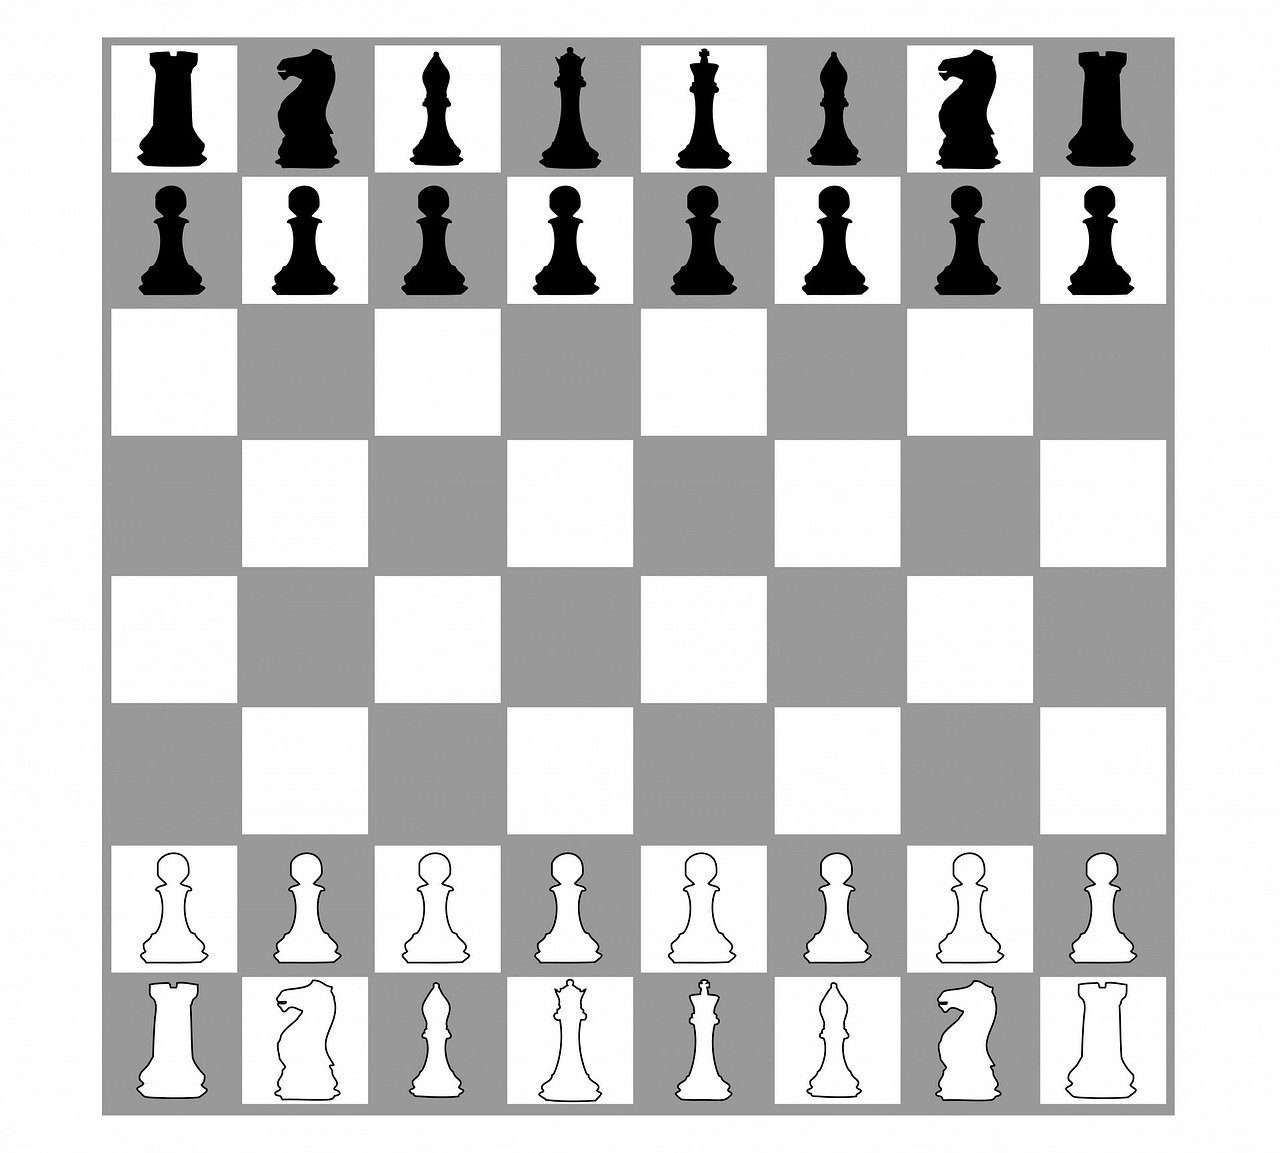
\includegraphics[scale=0.15]{chessBoard.jpg}
    \end{minipage}\hfill
    \begin{minipage}[H]{0.50\linewidth}
        \centering
        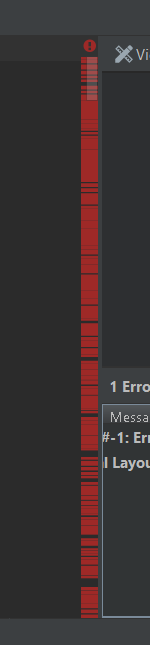
\includegraphics[scale=0.30]{echecbug.png}
    \end{minipage}\hfill
  \end{figure}
\end{frame}

\begin{frame}
    \frametitle{Jeu Snake}
    Jeu de snake de Google
    \begin{figure}
  	\begin{minipage}[H]{0.5\linewidth}
        \centering
        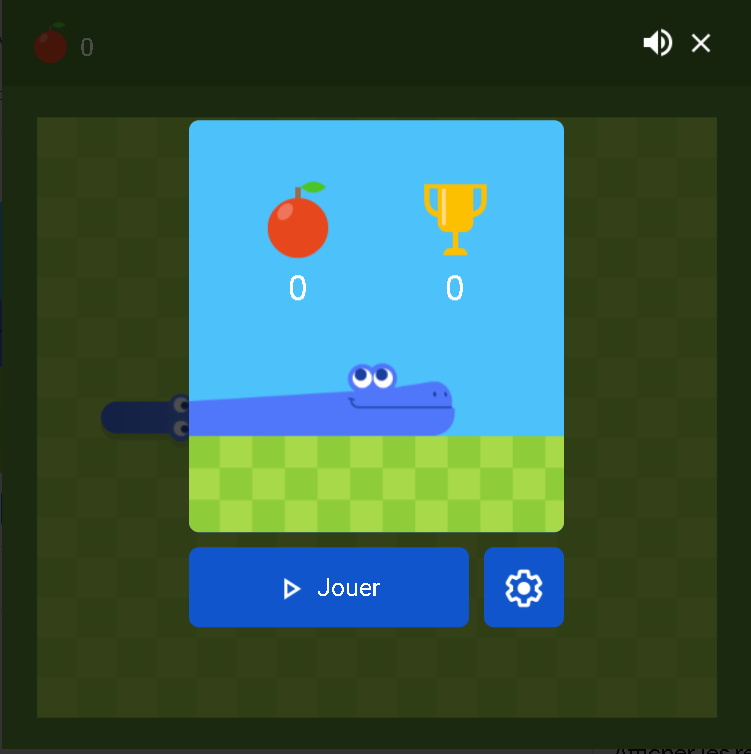
\includegraphics[scale=0.30]{MenuGoogleSnake.png}
    \end{minipage}\hfill
    \begin{minipage}[H]{0.50\linewidth}
        \centering
        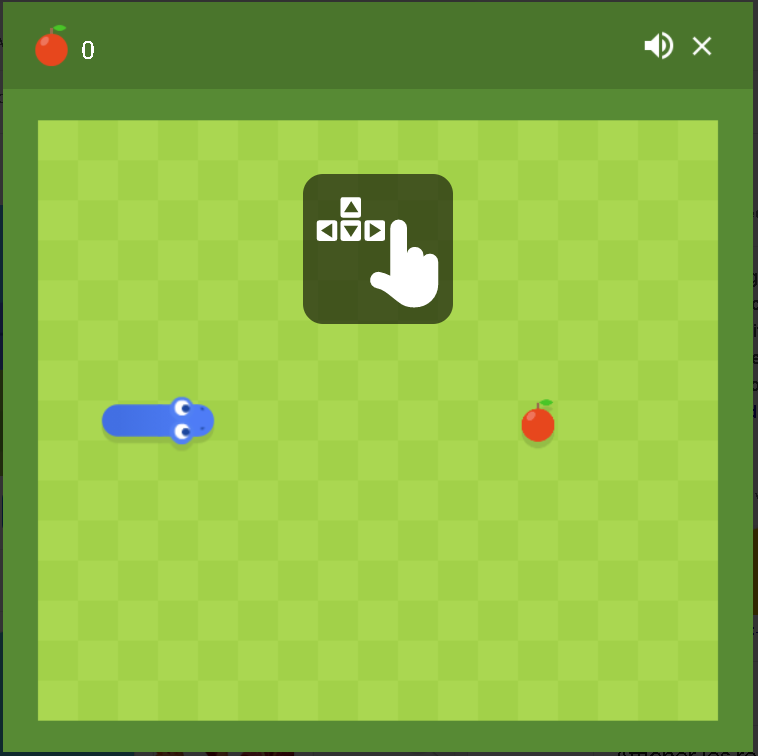
\includegraphics[scale=0.30]{JeuGoogleSnake.png}
    \end{minipage}\hfill
  \end{figure}
    
\end{frame}

%%%%%%%%%%%%%%%%%%%%%%%%%%%%%%%%%%%%
\section{Application Android}
%%%%%%%%%%%%%%%%%%%%%%%%%%%%%%%%%%%%
%
%
\begin{frame}{Notre jeu}
Notre touche personnelle :
    \begin{figure}[H]
    \begin{minipage}[H]{0.25\linewidth}
        \centering
        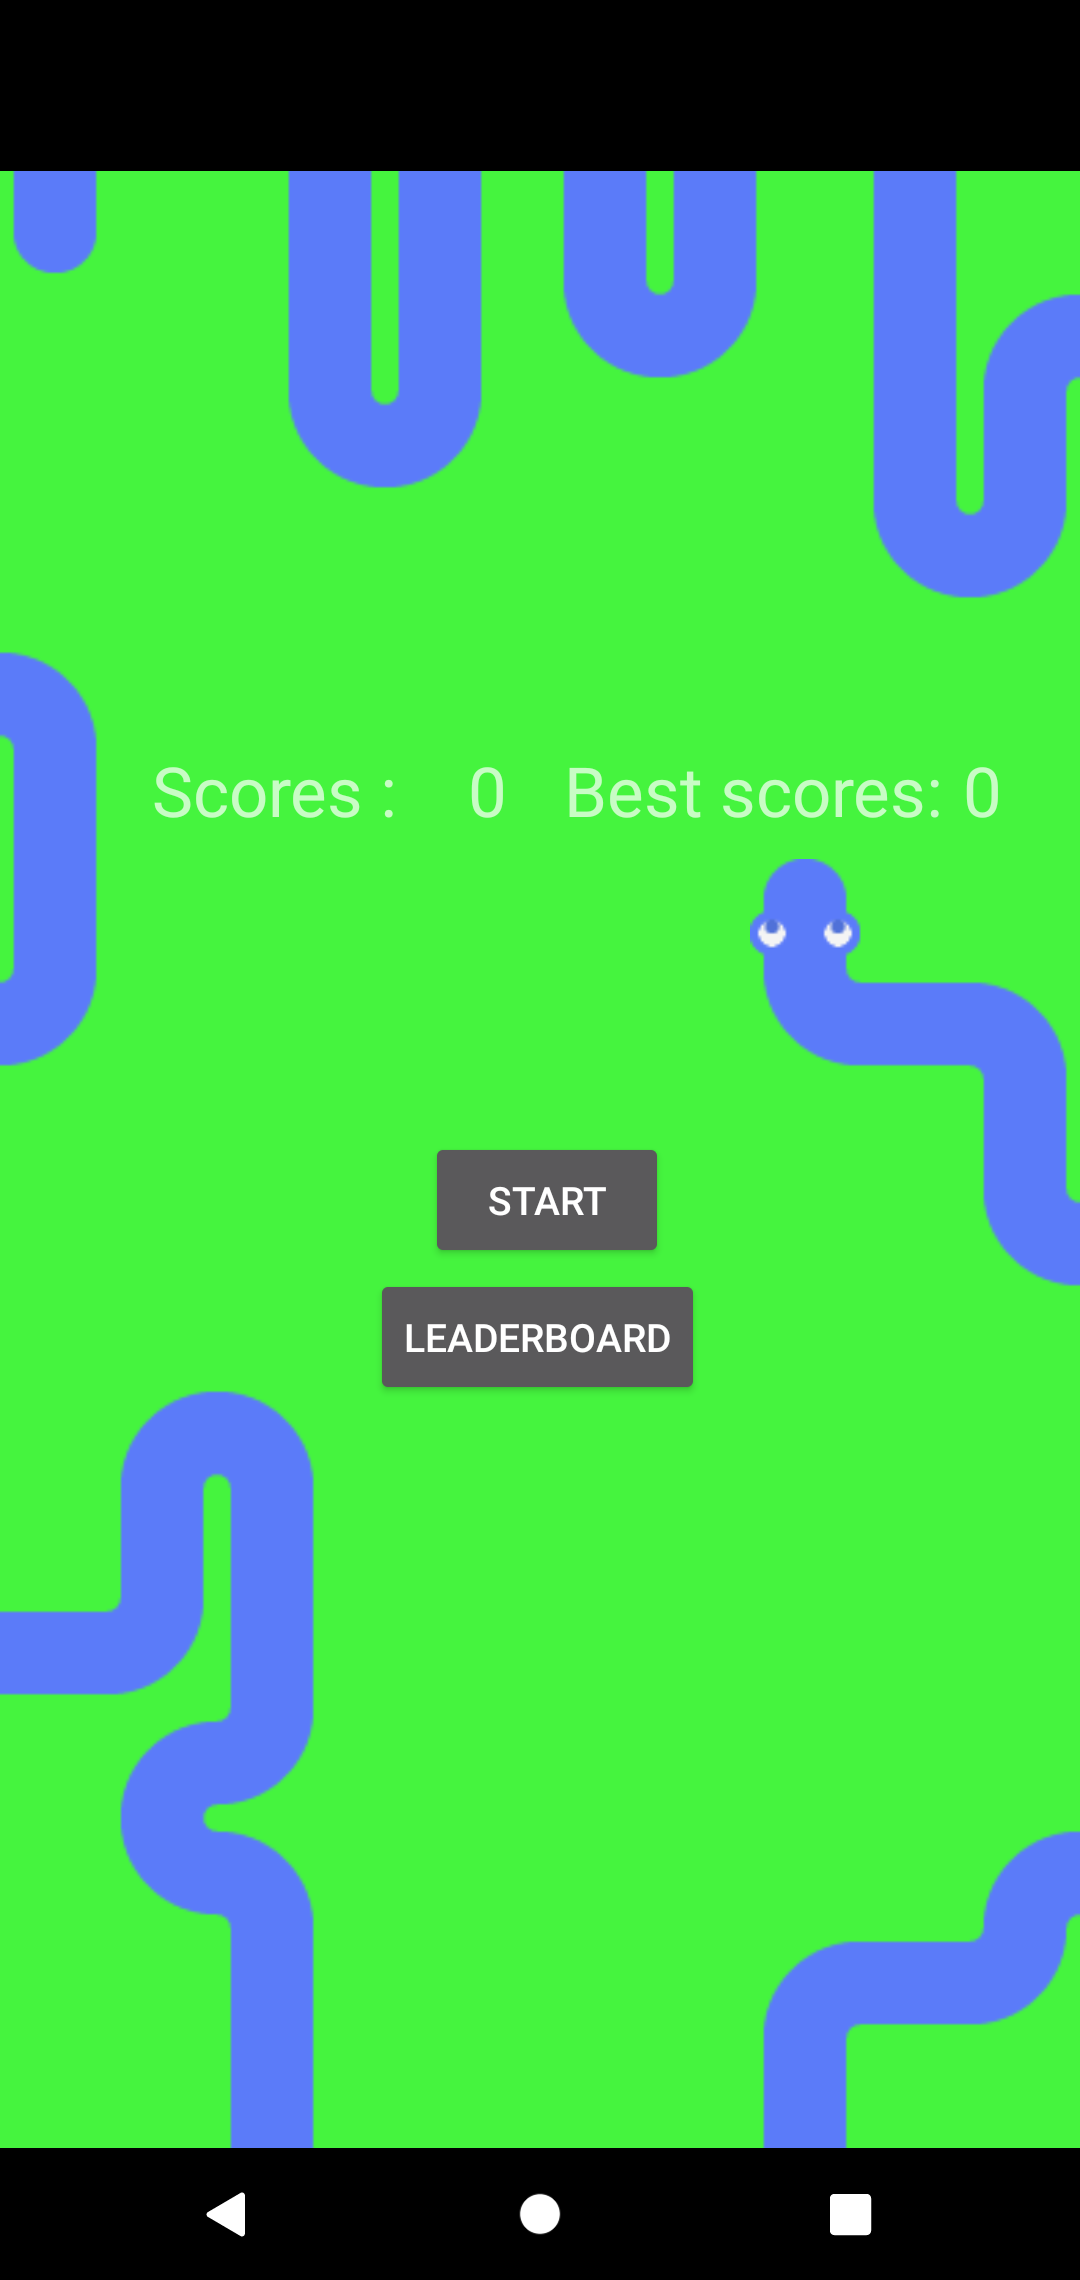
\includegraphics[scale=0.05]{MenuActi.png}
    \end{minipage}\hfill
    \begin{minipage}[H]{0.25\linewidth}
        \centering
        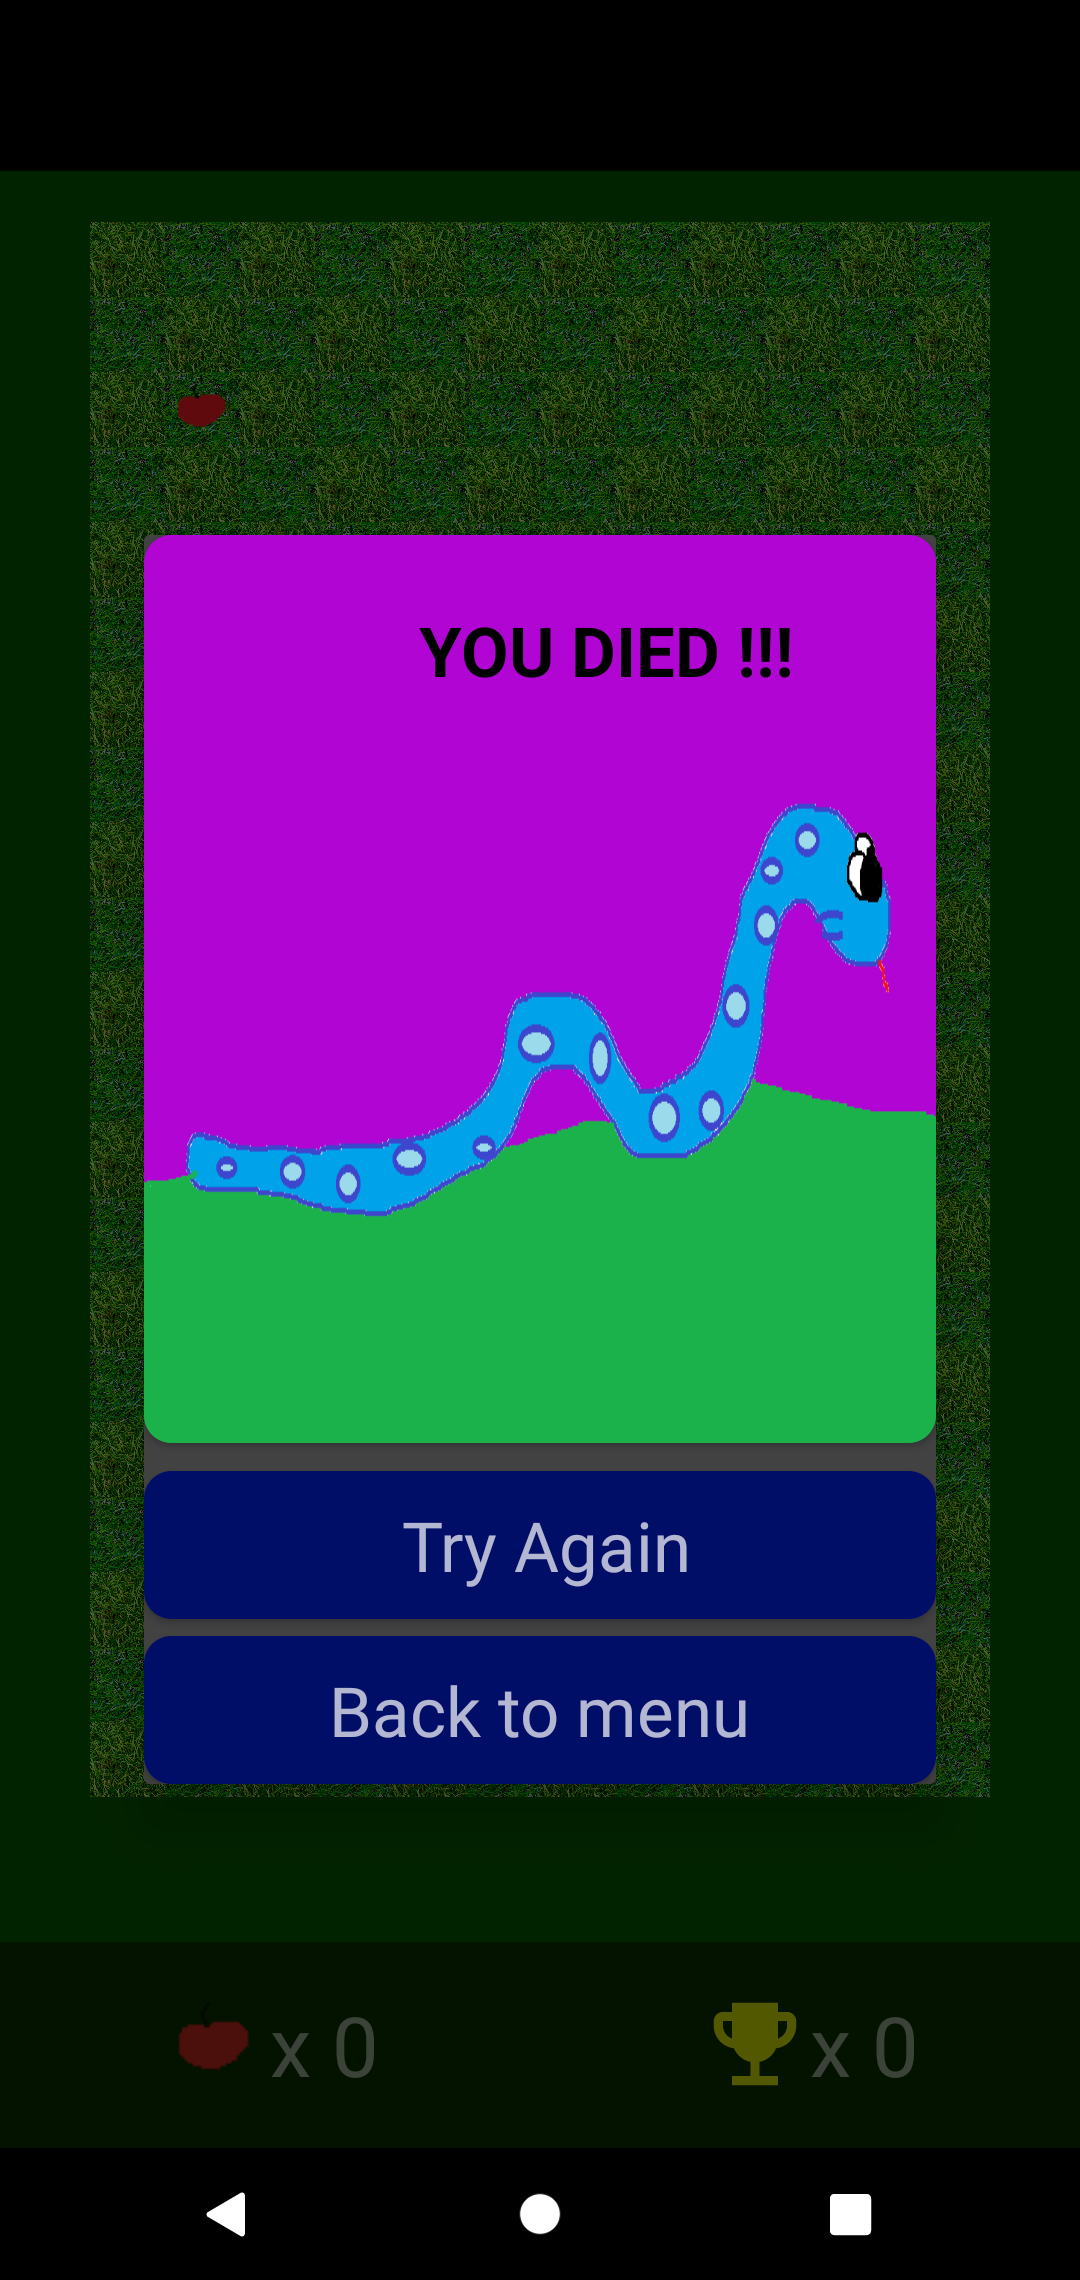
\includegraphics[scale=0.05]{MenuEnJeu.png}
    \end{minipage}\hfill
    \begin{minipage}[H]{0.25\linewidth}
        \centering
        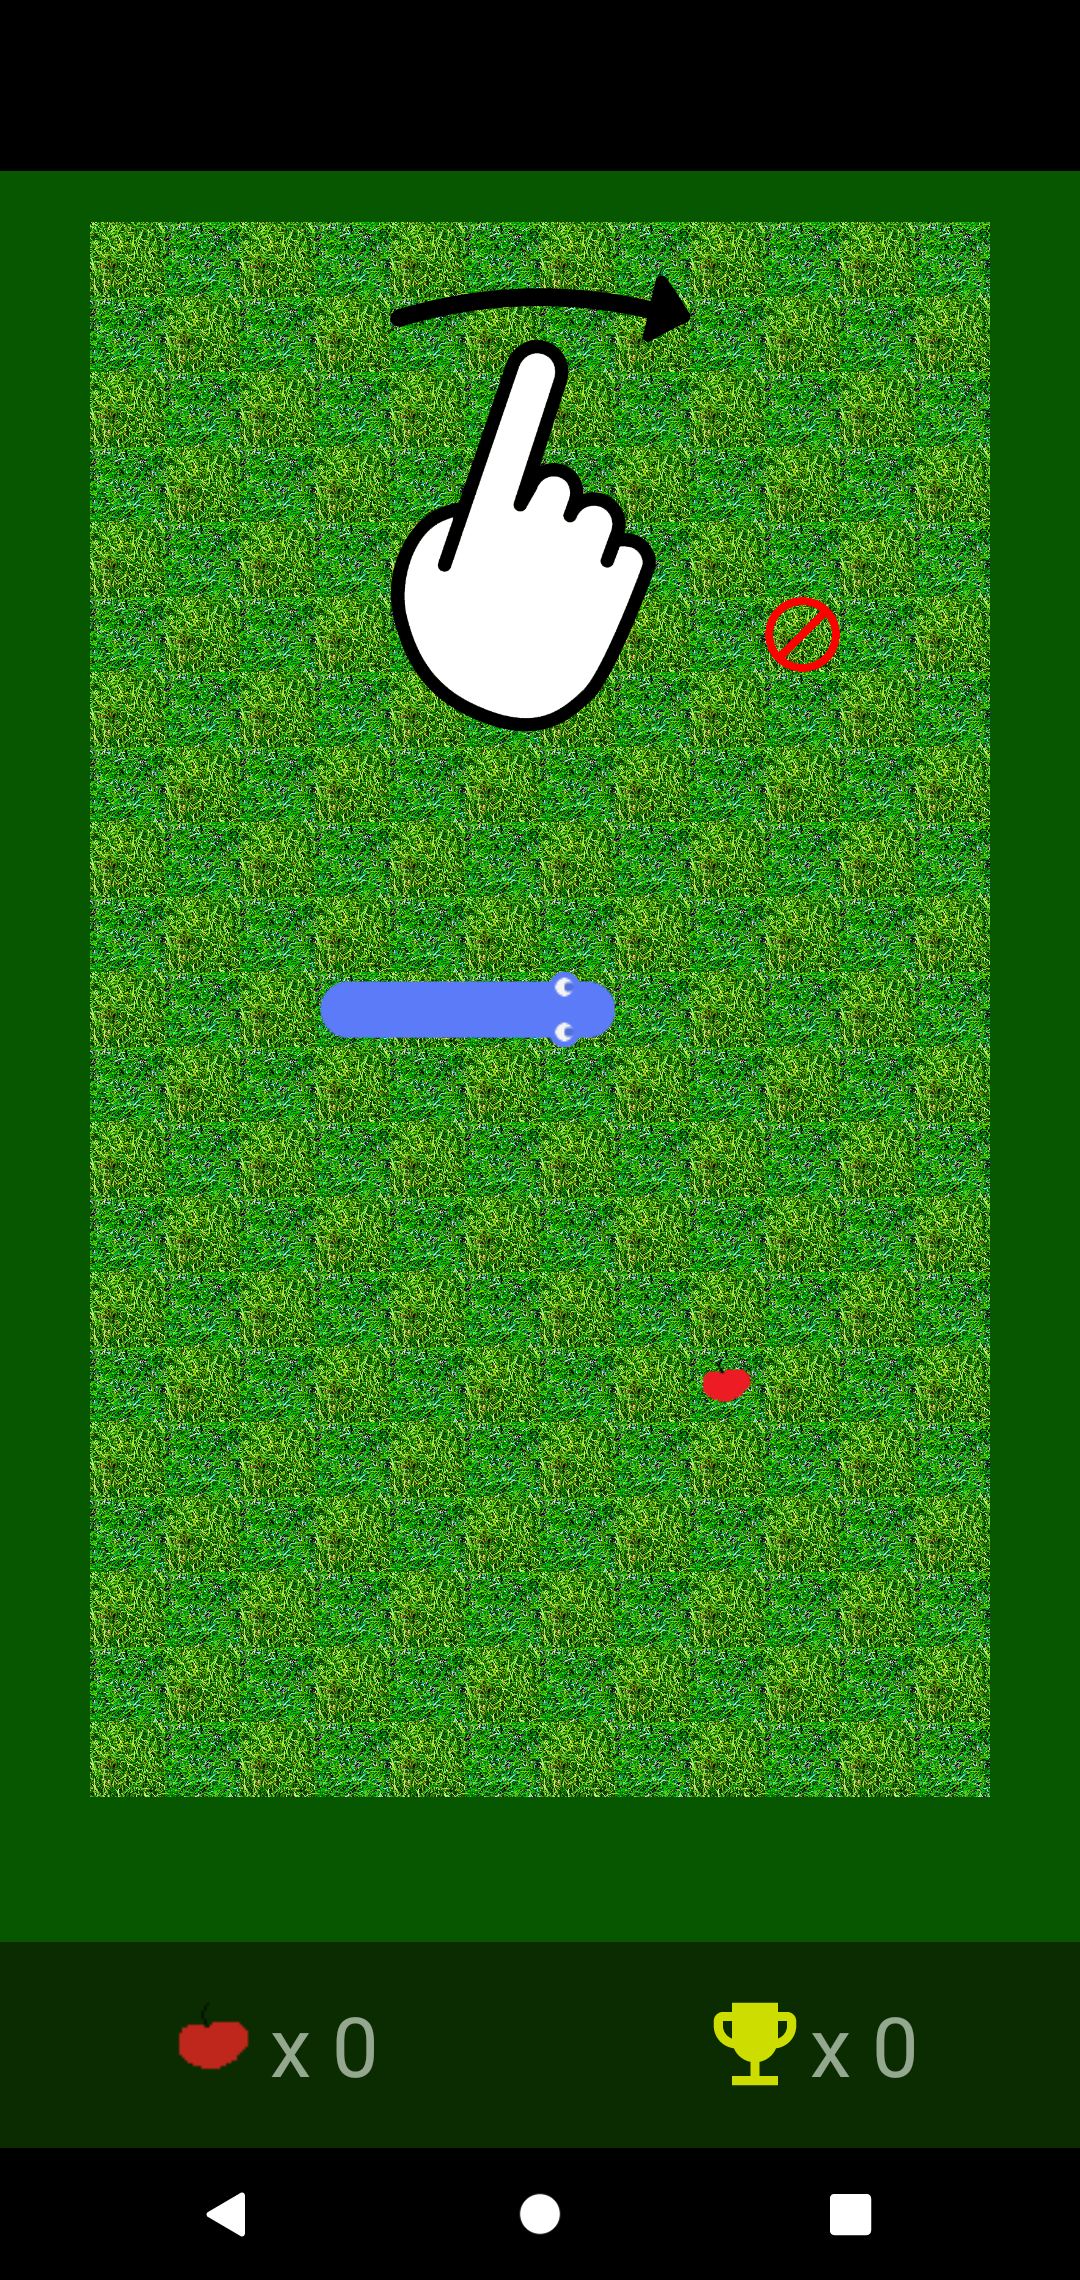
\includegraphics[scale=0.05]{Jeu.png}
    \end{minipage}\hfill
    \begin{minipage}[H]{0.25\linewidth}
        \centering
        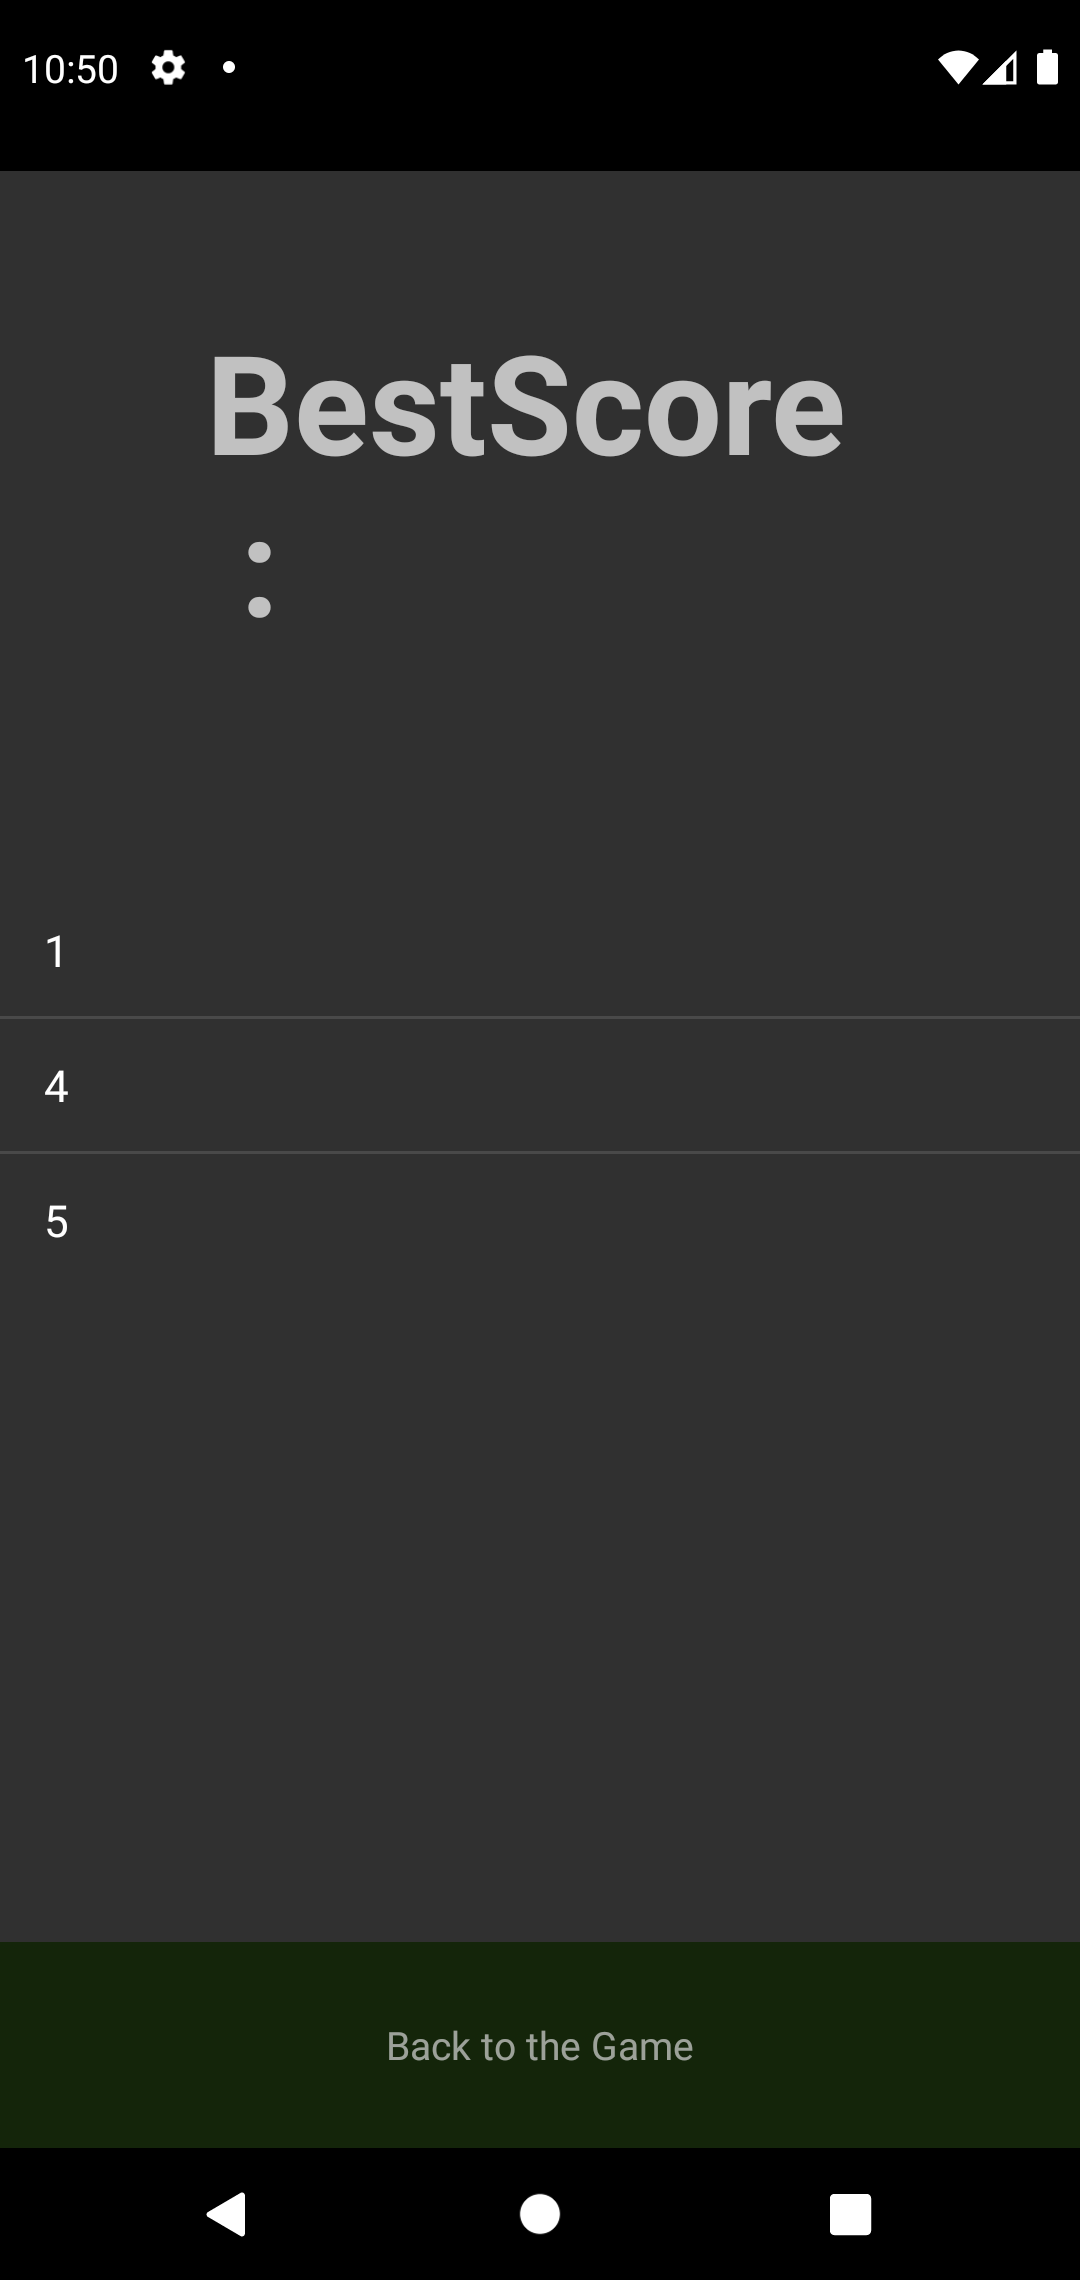
\includegraphics[scale=0.05]{LeaderBoard.png}
    \end{minipage}
    \end{figure}
\end{frame}

%
%
\begin{frame}{Logique du jeu}
  Le but du jeu est de contrôler un serpent afin de manger des pommes et d'esquiver les obstacles pour obtenir le meilleur score.
\end{frame}
%
%
\begin{frame}{Le Snake}
Création de l'objet snake :
    \begin{figure}
        \includegraphics[scale=0.4]{snake.png}
    \end{figure}
\end{frame}

\begin{frame}{Le Snake}
Update du snake :
    \begin{figure}
        \centering
        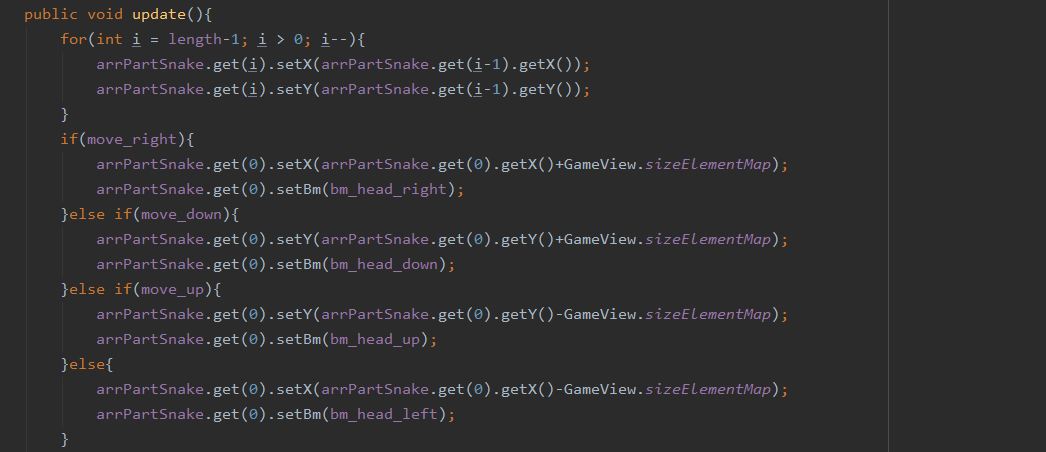
\includegraphics[scale=0.5]{updateSnake1.png}
\end{figure}
\end{frame}

\begin{frame}{Le Snake}
Update du snake (suite) :
    \begin{figure}
        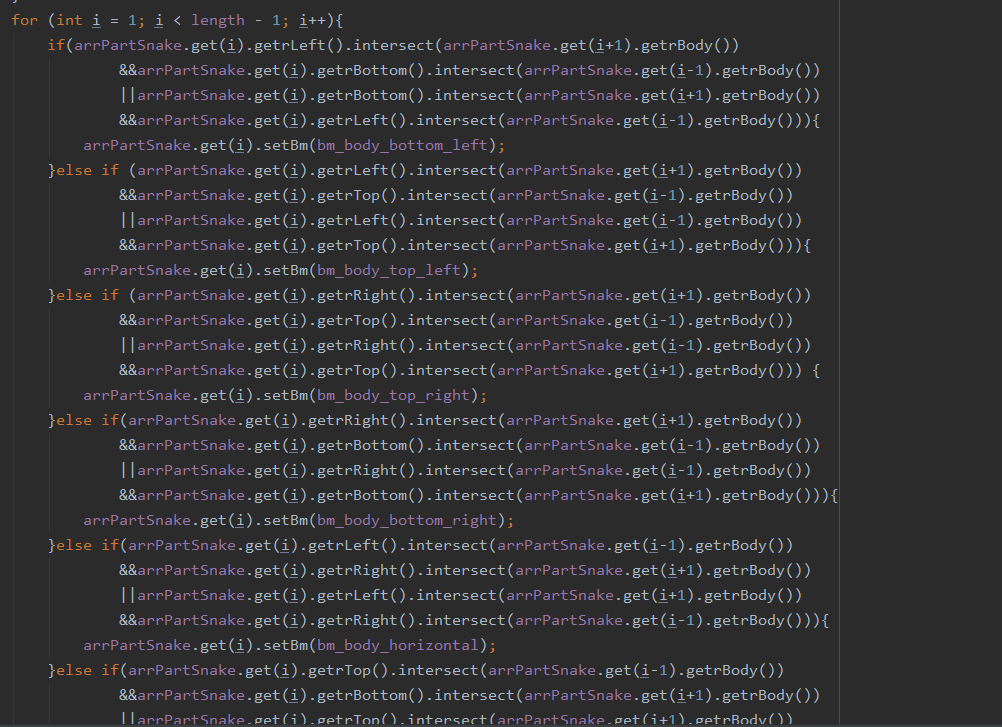
\includegraphics[scale=0.4]{UpdateSnake2.png}
    \end{figure}
\end{frame}

\begin{frame}{Le Snake}
Update du snake (suite) :
    \begin{figure}
        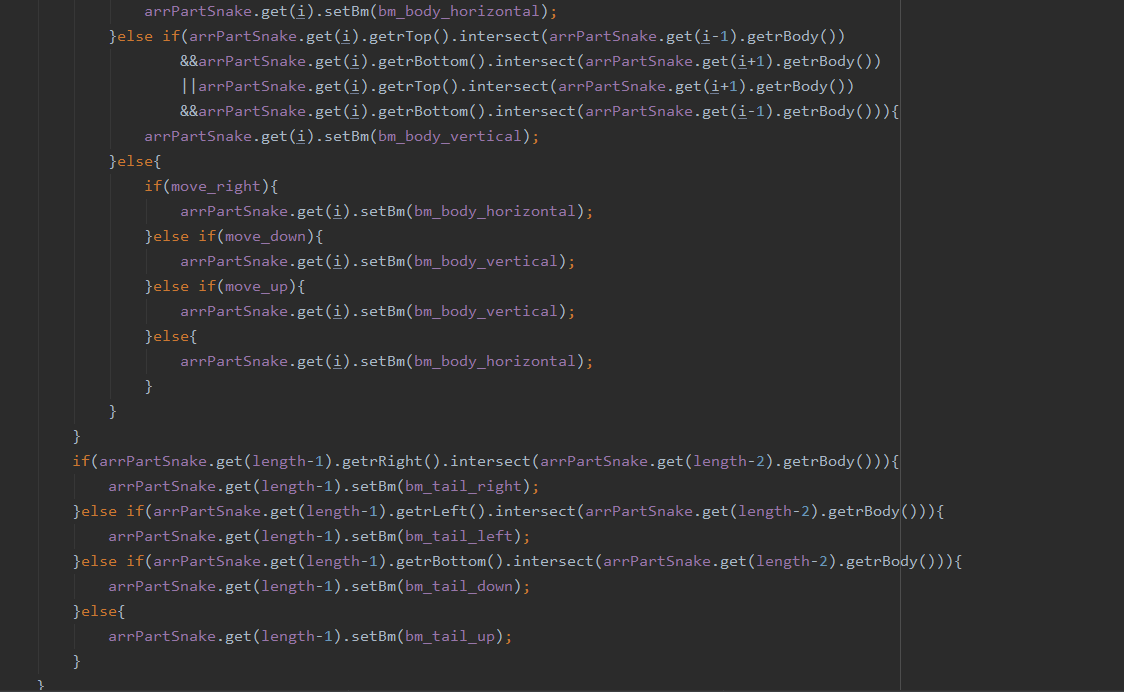
\includegraphics[scale=0.4]{UpdateSnake3.png}
    \end{figure}
\end{frame}

%
%
\begin{frame}{Passage entre les activités}
    Utilisation des OnClickListener sur bouton afin de naviguer entre les activités :
    \begin{figure}
    \begin{minipage}[H]{0.5\linewidth}
        \centering
        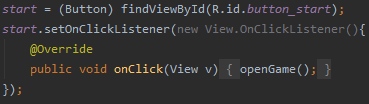
\includegraphics[scale=0.5]{OnClickButtons.png}
    \end{minipage}
    \begin{minipage}[H]{0.5\linewidth}
        \centering
        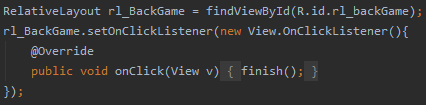
\includegraphics[scale=0.5]{OnClickRelativeLayout.png}
    \end{minipage}
    \end{figure}
\end{frame}

\begin{frame}{Passage entre les activités}
    Nos boutons et layouts de déplacements entre activités :
    \begin{figure}
    \begin{minipage}[H]{0.5\linewidth}
        \centering
        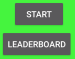
\includegraphics[scale=0.9]{ButtonsChangeActi.png}
    \end{minipage}\hfill
    \begin{minipage}[H]{0.5\linewidth}
        \centering
        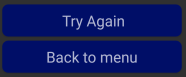
\includegraphics[scale=0.7]{LayoutChangeActi.png}
    \end{minipage}
    \end{figure}
\end{frame}
%
%
\begin{frame}{Le menu}
  Affichage du score et lien permettant d'accéder au leaderboard et du jeu principal :
  \begin{figure}
      \centering
      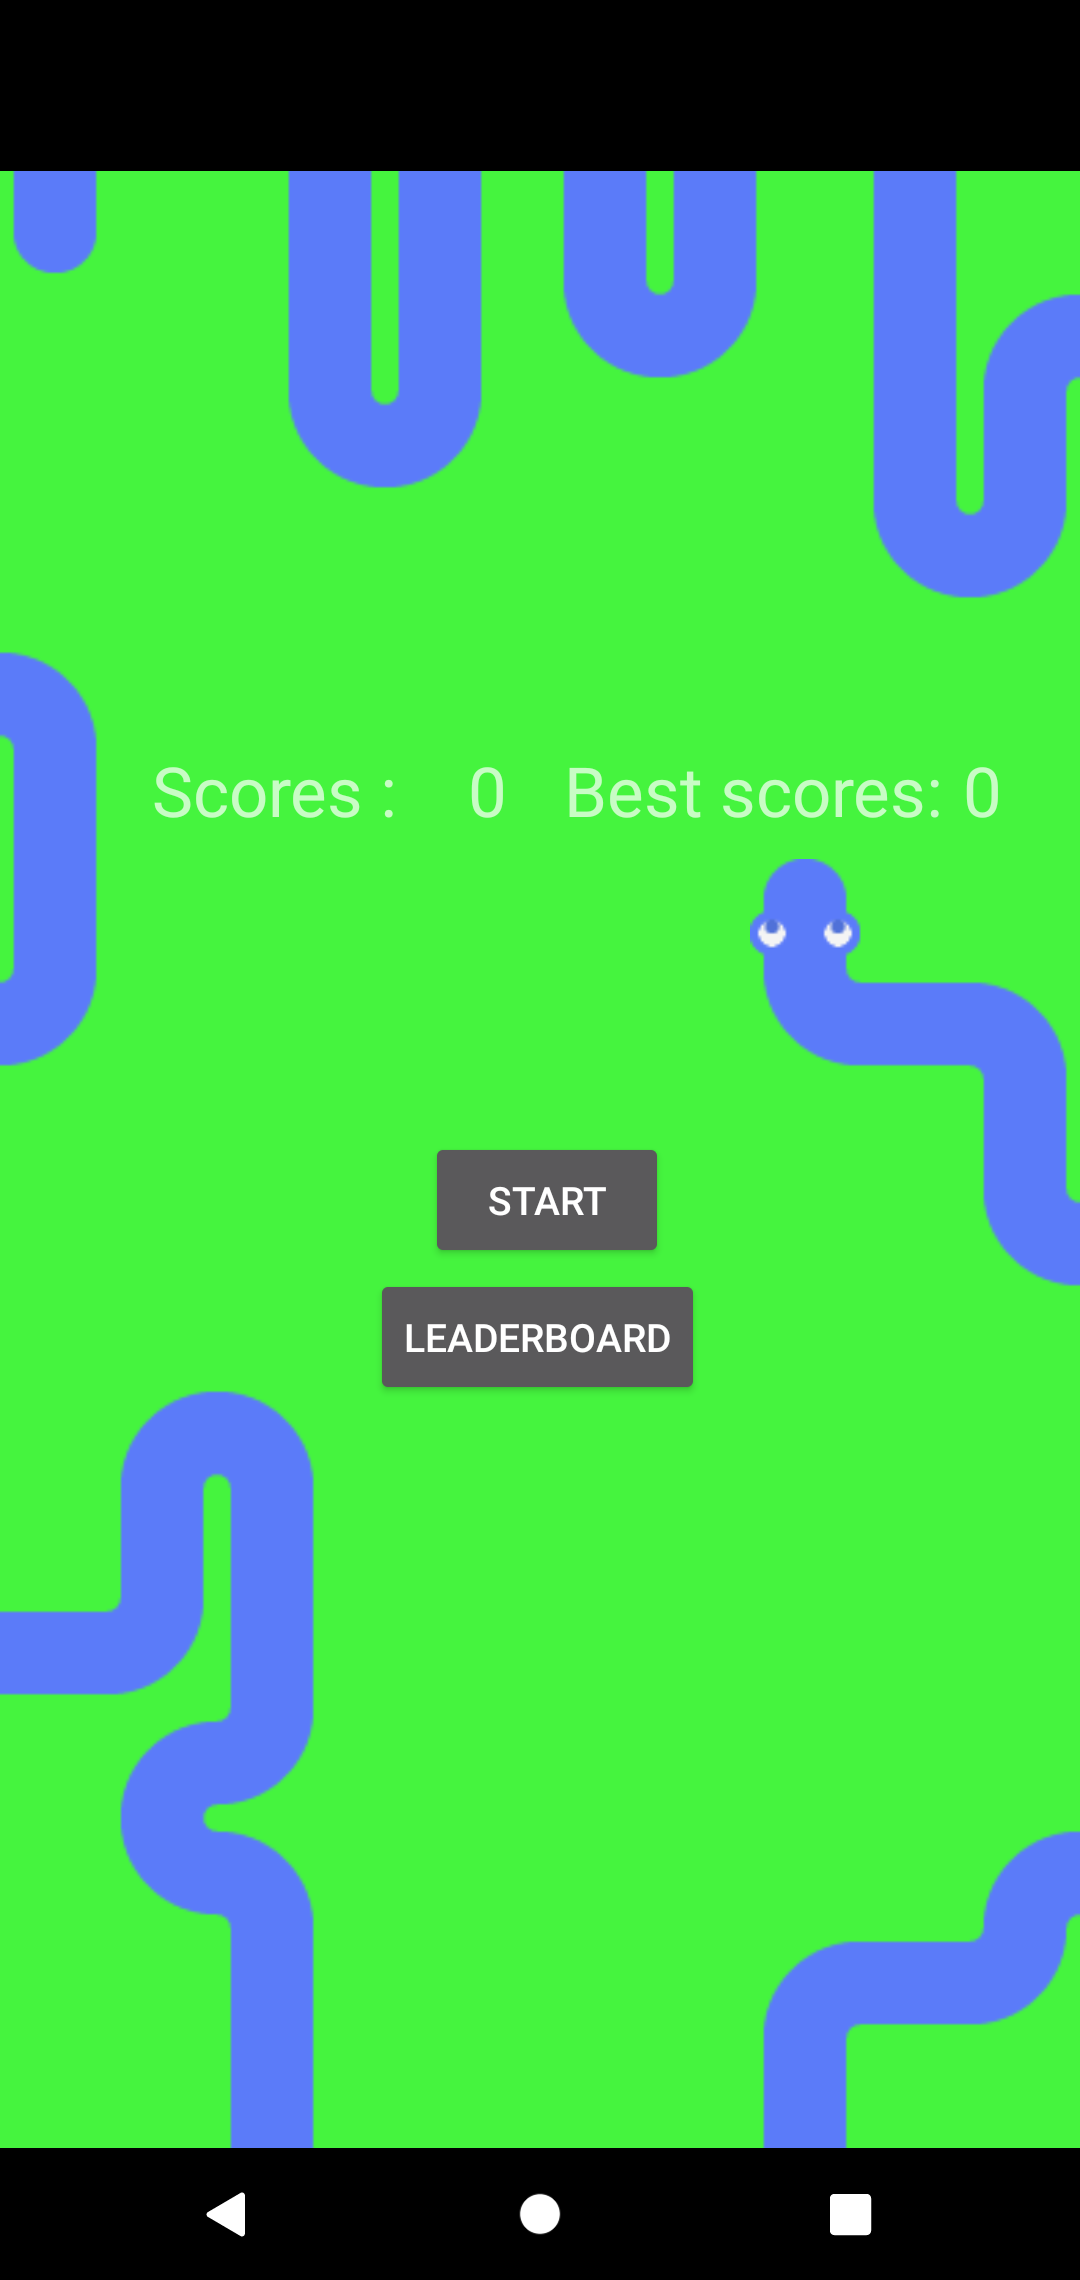
\includegraphics[scale=0.07]{MenuActi.png}
  \end{figure}
\end{frame}
%
%
\begin{frame}{La zone du jeu}
Dessin de texture sur un canvas
\begin{figure}
	\begin{minipage}[H]{0.33\linewidth}
        \centering
        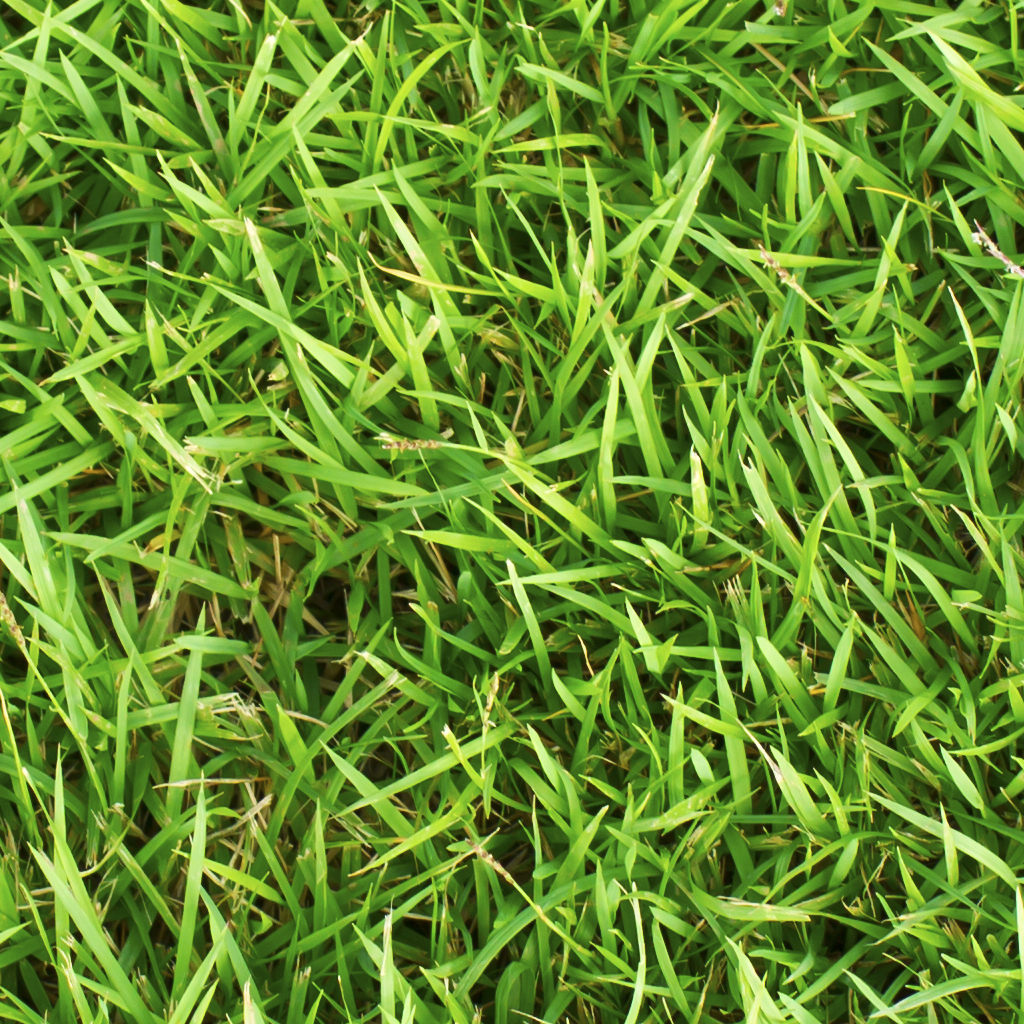
\includegraphics[scale=0.20]{texture_grass_1.png}
    \end{minipage}\hfill
    \begin{minipage}[H]{0.33\linewidth}
    	\centering
        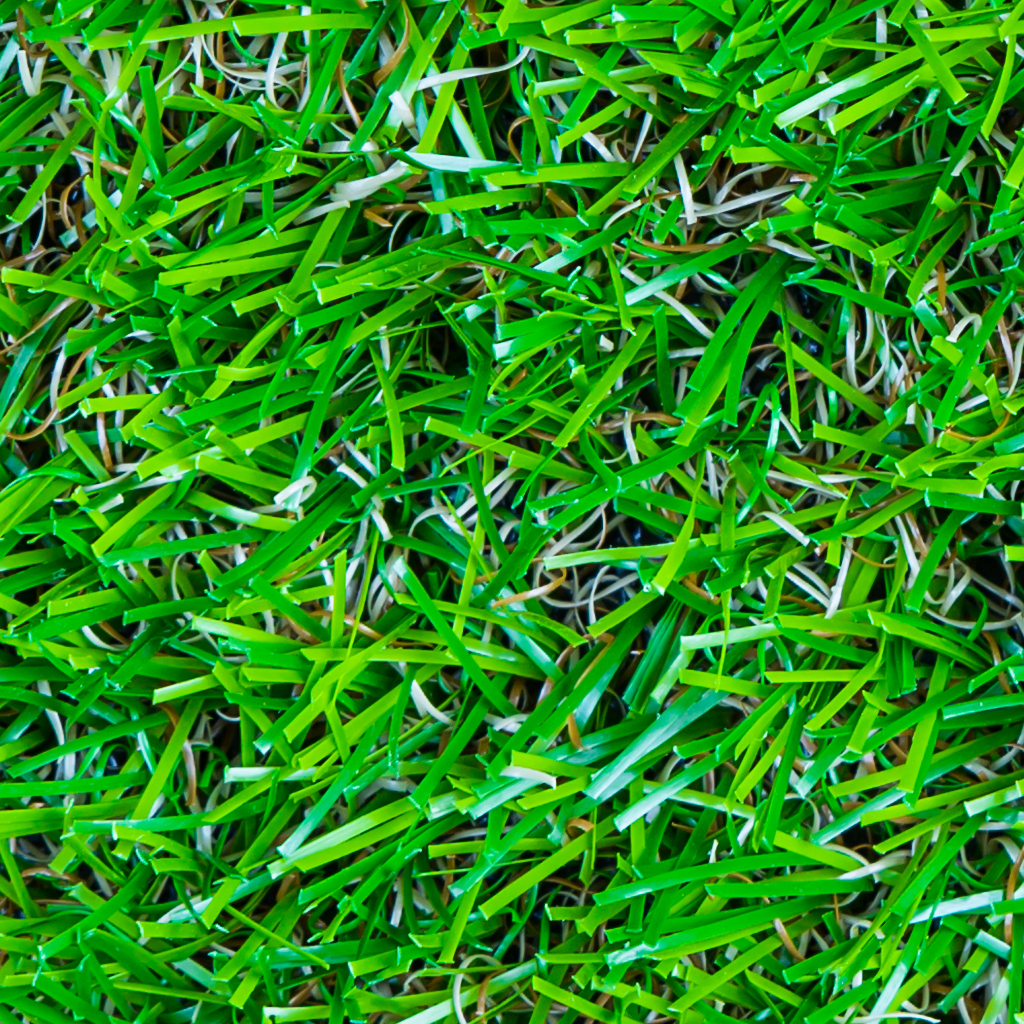
\includegraphics[scale=0.20]{texture_grass_2.png}
    \end{minipage}\hfill
    \begin{minipage}[H]{0.33\linewidth}
    	\centering
        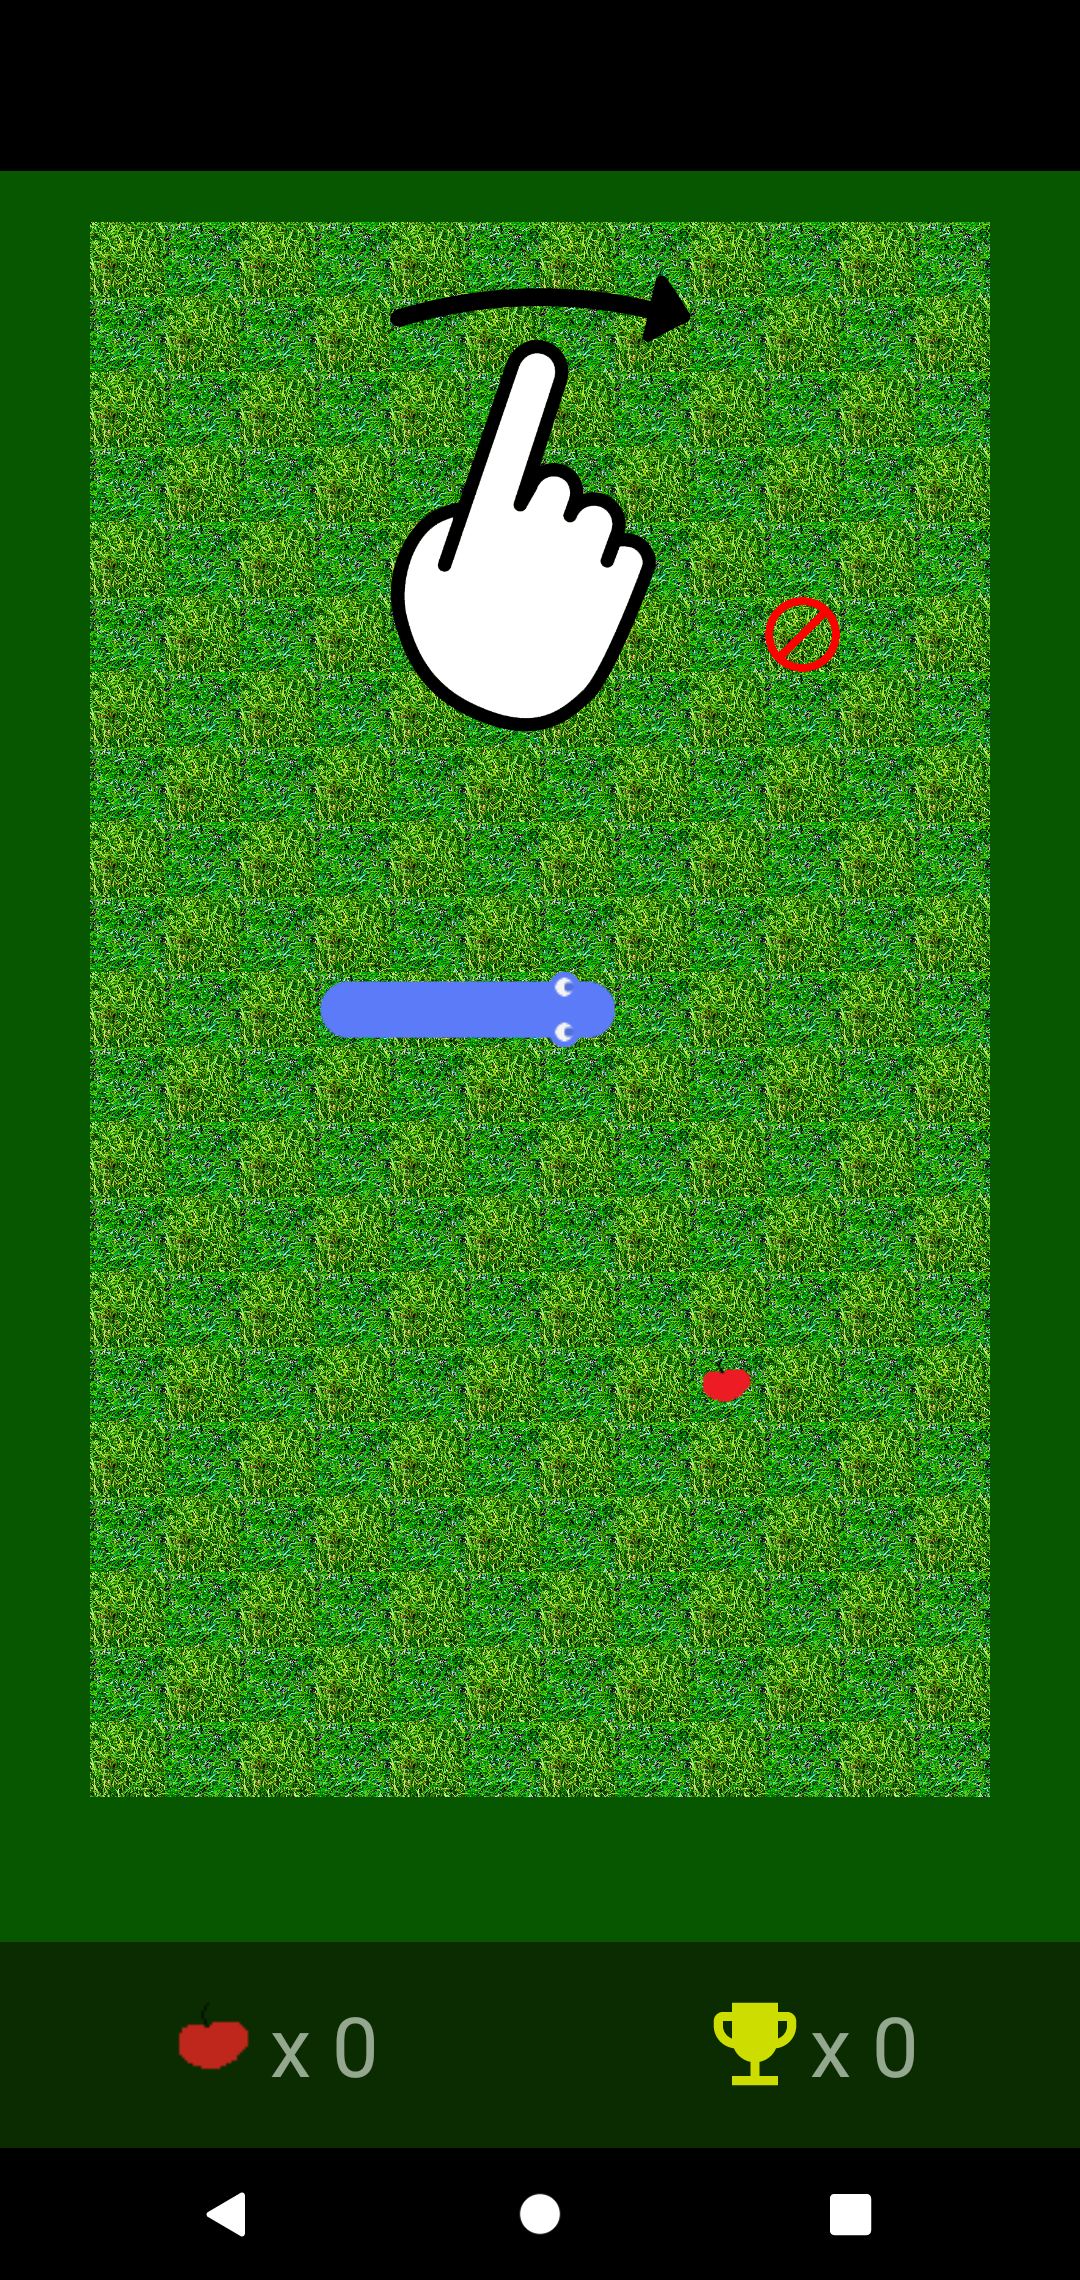
\includegraphics[scale=0.08]{Jeu.png}
    \end{minipage}\hfill
\end{figure}
\end{frame}
%
\begin{frame}{Gestion du stop}
Gestion du repositionnement toutes les x secondes du stop sur l'écran.
\begin{figure}
        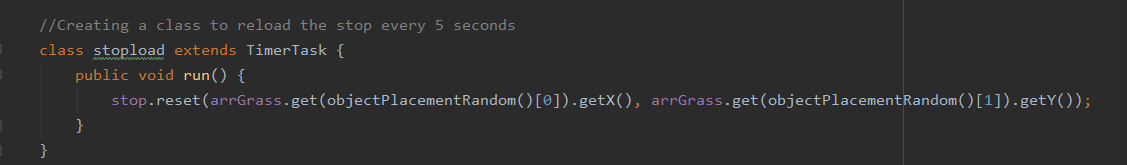
\includegraphics[scale=0.5]{stoptimer.png}
    \end{figure}
\end{frame}
%
\begin{frame}{Sauvegarde des données}
    Récupération des données de scores dans une Liste à la fin de chaque partie.
    \begin{figure}
        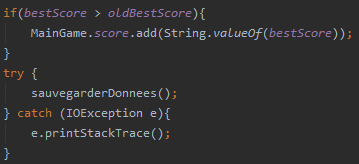
\includegraphics[scale=0.8]{SaveGameOver.png}
    \end{figure}
\end{frame}

\begin{frame}{Sauvegarde des données}
    Fonction de sauvegarde dans un fichier :
    \begin{figure}
        \centering
        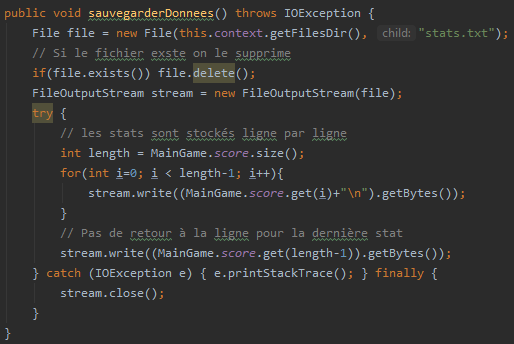
\includegraphics[scale=0.6]{SaveData.png}
    \end{figure}
\end{frame}

\begin{frame}{Sauvegarde des données}
    Fonction de chargement du fichier :
    \begin{figure}
        \centering
        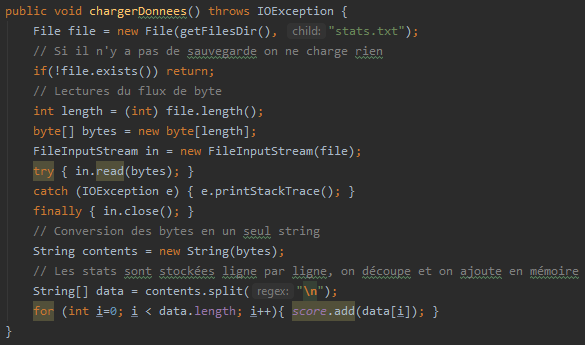
\includegraphics[scale=0.6]{LoadData.png}
    \end{figure}
\end{frame}
\begin{frame}{Sauvegarde des données}
Sauvegarde du meilleur dernier meilleur score dans les sharedPreferences
\begin{figure}
    \centering
    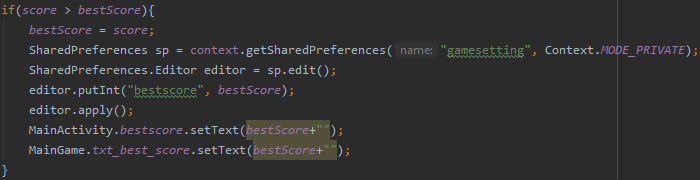
\includegraphics[scale=0.6]{SharedPreferences.png}
\end{figure}
\end{frame}
%
%
\begin{frame}{Affichage de la liste des meilleurs scores}
    Affichage sur une activité des différents meilleurs scores obtenu depuis l'ouverture du jeu sous forme de liste.
    \begin{figure}
        \begin{minipage}[C]{0.5\linewidth}
            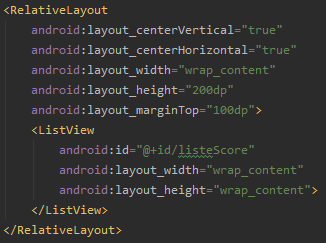
\includegraphics[scale=0.5]{RlLV.png}
        \end{minipage}\hfill
        \begin{minipage}[C]{0.5\linewidth}
            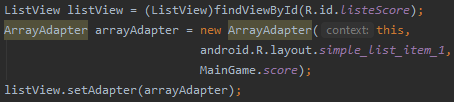
\includegraphics[scale=0.5]{CodeListView.png}
        \end{minipage}
    \end{figure}
\end{frame}

\begin{frame}{Affichage de la liste des meilleurs scores}
Résultat :
    \begin{figure}
        \centering
        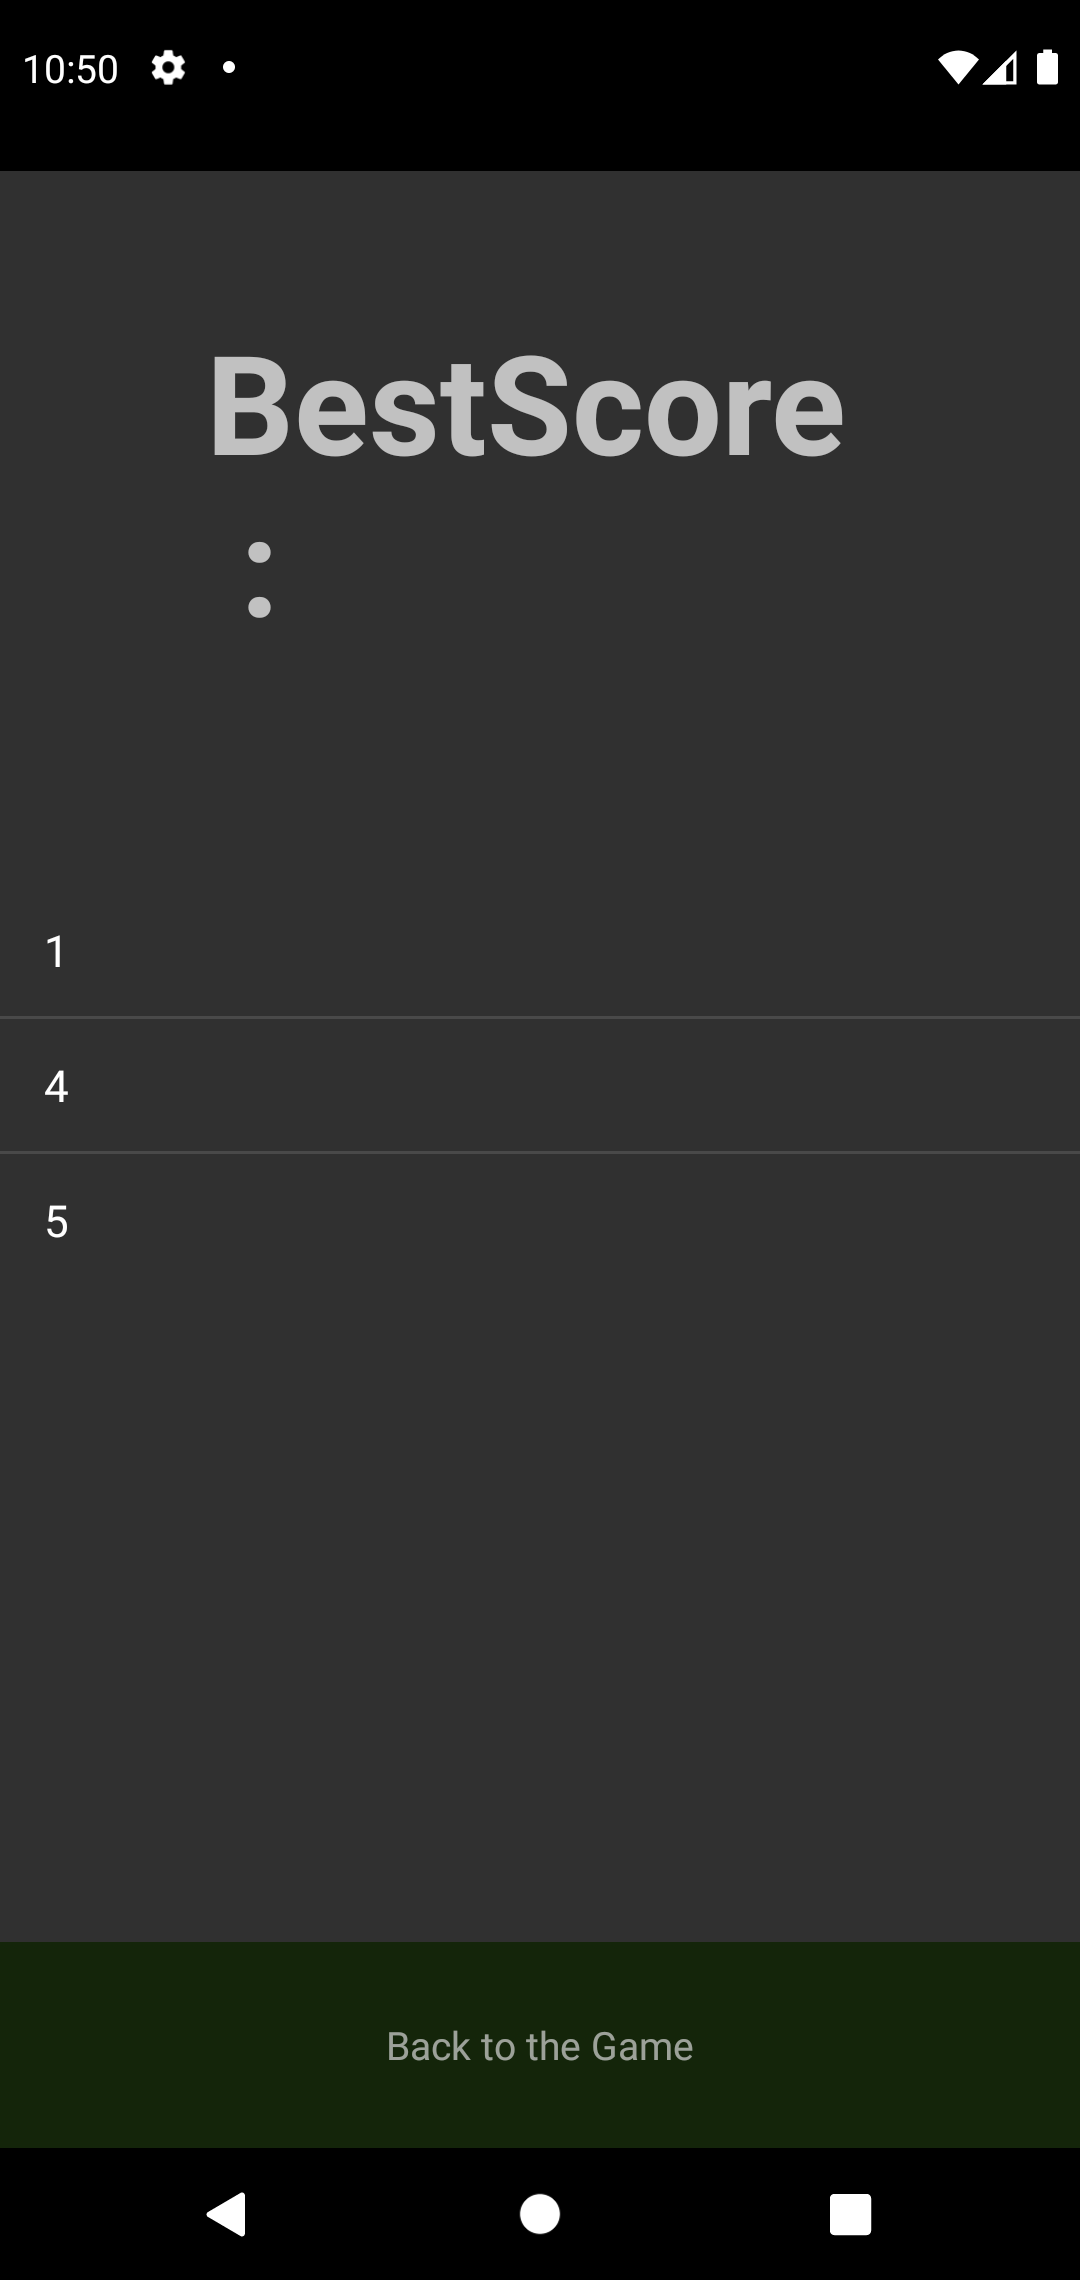
\includegraphics[scale=0.08]{LeaderBoard.png}
    \end{figure}
\end{frame}



%%%%%%%%%%%%%%%%%%%%%%%%%%%%%%%%%%%%
\section{Application iOS}

%%%%%%%%%%%%%%%%%%%%%%%%%%%%%%%%%%%%
%
%
\begin{frame}
  \frametitle{Logique du jeu}
	Le même que Android mais avec un déplacement par bouton.
\end{frame}
%
%
\begin{frame}{La zone de jeu}
Création d'un tableau de x*y case qui représente le boardgame
\begin{figure}
        \centering
        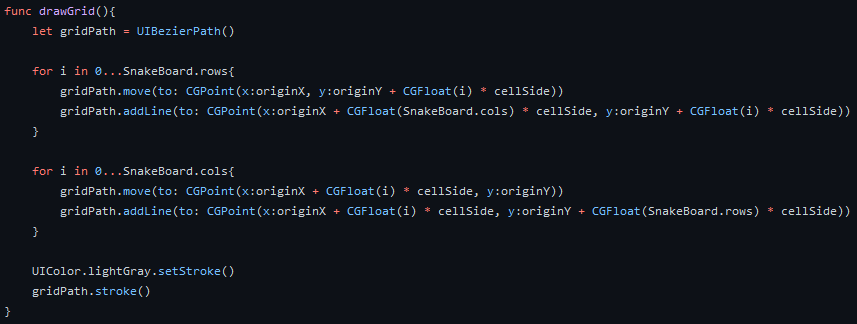
\includegraphics[scale=0.5]{DrawGrid.png}
    \end{figure}
\end{frame}
  
\begin{frame}
  \frametitle{Snake}
 Dessin de carrés représentants les différentes parties du serpent sur le boardgame.
 \begin{figure}
        \centering
        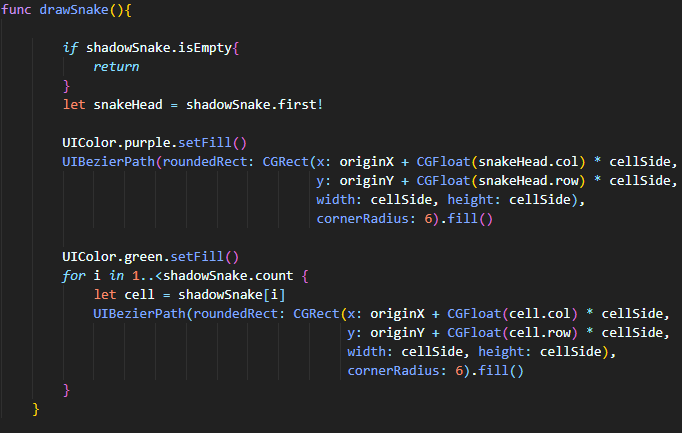
\includegraphics[scale=0.5]{DrawSnake.png}
    \end{figure}
  
\end{frame}

\begin{frame}
  \frametitle{Passage entre activité}
  Utilisation des UIViewController pour rediriger a l'aide d'un bouton.
  \begin{figure}
        \centering
        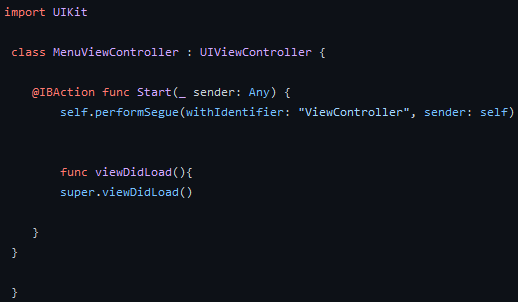
\includegraphics[scale=0.5]{MenuViewController.png}
    \end{figure}
\end{frame}
%
%
%%%%%%%%%%%%%%%%%%%%%%%%%%%%%%%%%%%%
\section{Contraintes}
%%%%%%%%%%%%%%%%%%%%%%%%%%%%%%%%%%%%
%
%
\begin{frame}{Contraintes}
La création de notre projet développement mobile a été ralentit lors de notre changement de sujet, impliquant plusieurs contraintes : 
\begin{itemize}
    \item De Temps
    \item De matériel
    \item La gestion de rotation d'écran
             \end{itemize}
\end{frame}
  
%
%
%%%%%%%%%%%%%%%%%%%%%%%%%%%%%%%%%%%%
\section{Bugs}
%%%%%%%%%%%%%%%%%%%%%%%%%%%%%%%%%%%%
%
%

\begin{frame}{Android}
  \begin{itemize}
    \item Le menu de mort au lancement du jeu
    \item Le leaderboard sans donnéesk
    \item La gestion de rotation d'écran
  \end{itemize}
\end{frame}
%
\begin{frame}{iOS}
  \begin{itemize}
    \item L'implémentation de la mort
    \item Le meilleurs scores
  \end{itemize}
\end{frame}
%
%
%%%%%%%%%%%%%%%%%%%%%%%%%%%%%%%%%%%%
\section{Conclusion}
%%%%%%%%%%%%%%%%%%%%%%%%%%%%%%%%%%%%
%
%
\begin{frame}
  \frametitle{Conclusion}
  \textbf{Pour conclure}
  \begin{itemize}
    \item
    \item
    \item
  \end{itemize}
\end{frame}
%
%
\end{document}
